\documentclass[11pt]{article}
\renewcommand{\rmdefault}{ptm}
\usepackage[scaled=0.92]{helvet}
\usepackage{courier,xcolor,colortbl,listings,parskip,graphicx,fancyvrb,fancyhdr,lastpage}
\usepackage{float,framed}
\normalfont
\usepackage[T1]{fontenc}
%\setlength{\parskip}{7pt}
\usepackage[toc,page]{appendix}
\usepackage[hmargin=2.5cm,vmargin=2cm]{geometry}
\usepackage[utf8]{inputenc}
\usepackage[brazil]{babel}
\usepackage{fancyvrb}
\pagestyle{fancy}
\setlength{\headheight}{120pt}
\setlength{\headsep}{30pt}
\setlength{\textheight}{550pt}
\renewcommand{\headrulewidth}{0pt}
\lhead{}
\rhead{}
\chead{
\includegraphics{brasao.jpg}\\
        \large \textbf{PRESIDÊNCIA DA REPÚBLICA}\\
        \large SECRETARIA-GERAL\\
        \large Secretaria-Executiva}
\cfoot{}
\rfoot{\thepage /\pageref{LastPage}}
\hyphenation{par-ti-ci-pa-ção}
\bibliographystyle{ieeetr}

\newcommand{\MyName}{Joenio Marques da Costa}
\newcommand{\MyEmail}{joenio@colivre.coop.br}
\newcommand{\ContractNumber}{2013/000564}
\newcommand{\ProjectCode}{Projeto PNUD BRA/12/018}
\newcommand{\NomeSecretaria}{Secretaria Geral da Presidência da República}
\newcommand{\SiglaSecretaria}{SG/PR}
\newcommand{\ProductNumber}{01}
\newcommand{\ProductDescription}{Documento com guia de codificação "coding
guidelines" para o desenvolvimento do código do portal objetivando o
reaproveitamento de código e o fomento à formação de comunidades em
torno dos módulos, bem como tutoriais para implementação local das
Soluções.
}
\newcommand{\MesEntrega}{Janeiro de 2014}
\newcommand{\DiaEntrega}{27}

\begin{document}
\lstset{language=Ruby}
\definecolor{light-gray}{gray}{0.95}
\lstdefinestyle{codeFrame}{backgroundcolor=\color{light-gray},frame=lines}

\textbf{\ProjectCode \ -} \ProductDescription

\vspace{3cm}

\begin{minipage}{0.5\textwidth}
  \textbf{Consultora: \MyName}
  \newline
  \textbf{Contrato nº: \ContractNumber}
  \newline
  \textbf{Produto / nº: \ProductNumber}
\end{minipage}

\vspace{2cm}

\textbf{Assinatura do Consultor}

\begin{framed}
Local e data: Brasília/DF, \line(1,0){20} \ de \line(1,0){100} \ de 2014
\newline
\newline
Assinatura do Consultor: \line(1,0){300}
\end{framed}

\vspace{1cm}

\textbf{Assinatura do Supervisor}

\begin{framed}
Atesto que os serviços foram prestados conforme estabelecido no Contrato
de Consultoria.
\newline
\newline
Local e data: Brasília/DF, \line(1,0){20} \ de \line(1,0){100} \ de 2014
\newline
\newline
Assinatura e Carimbo: \line(1,0){300}
\end{framed}

\clearpage
\newcolumntype{g}{>{\columncolor{light-gray}}l}

\begin{center}
  \begin{tabular}{| g | p{10cm} |}
    \hline
    \textbf{Título} & \ProductDescription \\ \hline
    \textbf{Língua do documento} & Português - Brasil \\ \hline
    \textbf{Documentação de referência} & Português \\ \hline
    \textbf{Unidade responsável} & \NomeSecretaria \
(\SiglaSecretaria) \\ \hline
    \textbf{Criador} & \MyName - \MyEmail \\ \hline
    \textbf{Taxonomias} & Desenvolvimento \\ \hline
    \textbf{Data de aprovação} & mês de ano \\ \hline
    \textbf{Público} & \SiglaSecretaria, Parceiros e Sociedade
Civil \\ \hline
    \textbf{Aplicabilidade} & Explicar isso aqui \\ \hline
    \textbf{Faz parte do} & \ProjectCode \\ \hline
    \textbf{Em conformidade com a} & \NomeSecretaria \\ \hline
    \textbf{Documentos anexos} & Nenhum \\ \hline
    \textbf{Revisado em} & dia mês ano \\ \hline
  \end{tabular}
\end{center}

\clearpage

\tableofcontents
\clearpage
\listoffigures

\clearpage

\section{Apresentação}

Em consonância com os objetivos e cronograma previsto no âmbito do
projeto BRA/12/018:
\textbf{Desenvolvimento de Metodologias de Articulação e Gestão de
Políticas Públicas para Promoção da Democracia Participativa},
firmado entre a Secretaria-Geral da Presidência da República
(SG/PR) e o Programa das Nações Unidas para o Desenvolvimento (PNUD),
o presente documento apresenta um guia de codificação "coding guidelines" para
o desenvolvimento do código do portal objetivando o reaproveitamento de código
e o fomento à formação de comunidades em torno dos módulos, bem como tutoriais
para implementação local das soluções.

Essa proposta está configurada como produto \ProductNumber~da consultoria técnica
para especificação da construção dos códigos das metodologias de
organização da informação e interação participativa do portal de
participação social.

\section{Comunidade Noosfero}

% http://noosfero.org/Site/CommunityPtbr

A comunidade de desenvolvimento do projeto Noosfero é organizada
ao redor de listas de discussão, salas de bate-papo no irc, ferramenta
tracker, repositório de código fonte e encontros e conferências.

A página da comunidade brasileira do projeto encontra-se no seguinte link,
onde são vinculadas notícias, notas de lançamentos, organização
de eventos, etc.

\begin{itemize}
  \item http://softwarelivre.org/noosfero
\end{itemize}

Além da página web da comunidade, a ferramenta de lista de discussão,
noosfero-br, é amplamente utilizada para discutir qualquer assunto
relevante ao projeto, seja de uso, seja relacionado ao desenvolvimento,
desde que seja no idioma português.

\begin{itemize}
  \item http://listas.softwarelivre.org/cgi-bin/mailman/listinfo/noosfero-br
\end{itemize}

Este é, sem dúvida, o melhor espaço para tirar dúvidas e propor melhorias
ao projeto Noosfero.

Para discussões em inglês, e este é o idioma preferível para discussões
técnicas e desenvolvimento do projeto, existe a lista noosfero-dev.

\begin{itemize}
  \item http://listas.softwarelivre.org/cgi-bin/mailman/listinfo/noosfero-dev
\end{itemize}

Qualquer pessoa pode se inscrever na lista de desenvolvimento.  O idioma desta
lista é o inglês. Se você quer discutir desenvolvimento mas não se sente à
vontade com o inglês, use a lista noosfero-br.

Outra forma de comunicação adotada pela comunidade Noosfero
é o IRC, através dos seguintes canais na rede Freenode (irc.freenode.net).

\begin{itemize}
  \item \#noosfero-br: discussão em português
  \item \#noosfero: discussão em inglês (desenvolvimento)
\end{itemize}

Você pode ainda obter informações sobre a comunidade e o projeto Noosfero
através do Ohloh\footnote{http://www.ohloh.net/projects/noosfero}, como
demonstrado na figura~\ref{fig:noosfero-ohloh}.

\begin{figure}[h]
\center
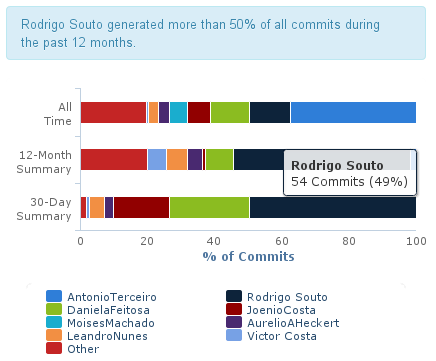
\includegraphics[scale=0.5]{noosfero-ohloh.png}
\caption{Estatísticas da comunidade Noosfero no Ohloh}
\label{fig:noosfero-ohloh}
\end{figure}

\section{Desenvolvimento do Noosfero}

% http://noosfero.org/Development/GettingStartedWithNoosferoDevelopmentPt

\subsection{Obtendo o código-fonte}

Existem três formas básicas de obter o código fonte.

\subsubsection{Tarballs}

No endereço abaixo abra o tópico do release desejado e clique no arquivo da versão
para fazer o download.

\begin{itemize}
  \item http://noosfero.org/Development/MilestoneItems
\end{itemize}

\subsubsection{Diretamente do repositório git}

Este caminho é útil apenas para quem não quer ser um colaborador, mas quer o código
mais recente ainda em desenvolvimento.

\begin{Verbatim}[frame=single,fontfamily=courier]
  git clone https://gitlab.com/noosfero/noosfero.git
\end{Verbatim}

\subsubsection{Através de um fork no Gitlab}

Este é o {\bf melhor} caminho para quem quer contribuir com o Noosfero.

Você precisa fazer login no
Gitlab.com\footnote{https://gitlab.com/users/sign\_in}, acessar
https://gitlab.com/noosfero/noosfero e criar um fork do repositório clicando
em "Fork repository".

\begin{figure}[h]
\center
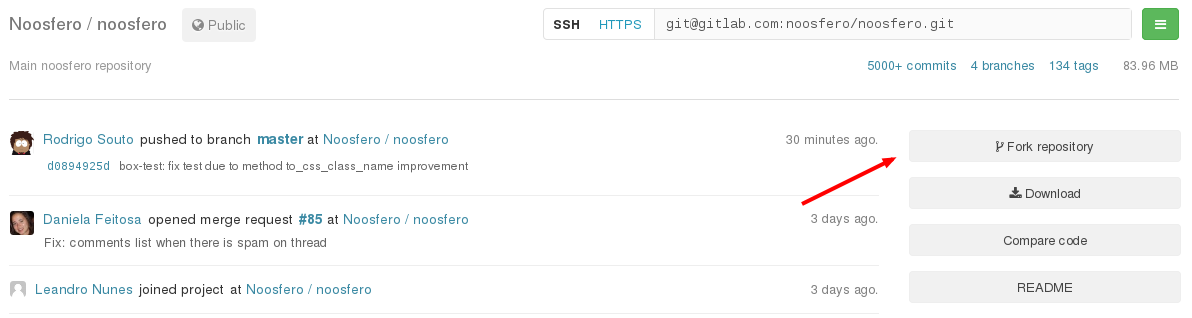
\includegraphics[scale=0.4]{gitlab-fork.png}
\caption{Criando fork do repositório no Gitlab}
\label{fig:gitlab-fork}
\end{figure}

Agora você pode baixar os fontes desse fork em seu computador e começar a trabalhar: 

\begin{figure}[h]
\center
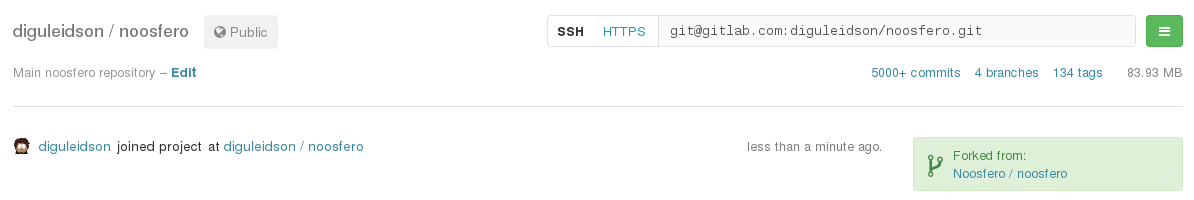
\includegraphics[scale=0.4]{gitlab-forked.png}
\caption{Fork local do repositório}
\label{fig:gitlab-forked}
\end{figure}

Após o fork no Gitlab faça o seguinte: 

\begin{Verbatim}[frame=single,fontfamily=courier]
  git clone https://gitlab.com/<username>/noosfero.git 
\end{Verbatim}

ou isso: 

\begin{Verbatim}[frame=single,fontfamily=courier]
  git clone git@gitlab.com:<username>/noosfero.git
\end{Verbatim}

Você precisa receber atualizações do repositório oficial, então registre-o
da seguinte forma:

\begin{Verbatim}[frame=single,fontfamily=courier]
  git remote add origin https://gitlab.com/noosfero/noosfero.git
\end{Verbatim}

Sempre que você quiser pode obter atualizações do repositório oficial
executando:

\begin{Verbatim}[frame=single,fontfamily=courier]
  git pull origin master
\end{Verbatim}

\subsection{Instalação, Execução, Desenvolvimento}

Se você é um usuário Debian, simplesmente rode {\it script/quick-start} a partir da
raiz do Noosfero. Isto irá preparar o seu ambiente automaticamente para
desenvolvimento.

Você vai precisar de alguns usuários, comunidades e dados de teste para interagir
enquanto desenvolve, então rode o {\it script/sample-data} e alguns dados de
exemplo serão criados.

Se você tem uma máquina GNU/Linux, mas não é um Debian Stable, você pode querer
usar um schroot\footnote{http://noosfero.org/Development/Schroot}. Não se
preocupe. Isso é fácil e vai salvar sua vida.

\section{Orientações para contribuição}

% http://noosfero.org/Development/PatchGuidelinesPt

\subsection{Criar ActionItem}

No menu esquerdo do tracker\footnote{http://noosfero.org/Development} do
Noosfero, use o 'Quick item creation' para descrever um novo bug ou
nova funcionalidade.

\subsection{Configurar um branch}

Crie um fork do repositório\footnote{https://gitlab.com/noosfero/noosfero.git}
noosfero oficial clicando em {\bf Fork repository}. Então adicione o repositório
remoto oficial:

\begin{Verbatim}[frame=single,fontfamily=courier]
  git remote add noosfero https://gitlab.com/noosfero/noosfero.git
  git fetch noosfero
  git checkout noosfero/stable -b aiXXXX
\end{Verbatim}

Se você está trabalhando em um bug, então use o {\it noosfero/stable} como base. Se
é uma funcionalidade, use {\it noosfero/master} como base.

Para facilitar a nomenclatura use o padrão {\it aiXXXX}, substituindo XXXX com o
respectivo número do ActionItem. Você também pode criar o seu próprio nome.

\subsection{Guia de codificação}

Tente sempre lembrar que outros irão ler e alterar o seu código.

\subsubsection{Princípios}

Tenha em mente estes importantes princípios.

{\bf Comunicar}

Inglês é a língua padrão para o desenvolvimento dos ActionItems, código,
commits e tudo o que envolve desenvolvimento. Isso ajuda os desenvolvedores de
todo o mundo a fazer parte da comunidade Noosfero.

Para commits e descrições de ActionItems, você não precisa usar termos
repetitivas como deve ou deveria. Basta colocar a frase na forma imperativa e
explicar os fatos observados e implementados.

Para commits, escreva um resumo compreensível para o seu patch, descrevendo o
que ele faz, não qual era o problema antes dele. Por exemplo, em vez de "Erro
ao fazer isso e aquilo", escreva "Corrigido erro ao fazer isso e aquilo".

{\bf Foco}

Concentre-se na mudança que você está fazendo e não misture com coisas não
relacionadas. Quanto menos foco uma certa modificação tem mais confuso se
torna o trabalho de revisão.

{\bf Agregar}

Agregue linhas de código com funções semanticamente semelhantes.

{\bf Encapsular}

Mesmo que o código seja pequeno, coloque-o em uma função adequada que tenha
significado e incentive a reutilização.

{\bf Escopo}

Mesmo que o seu código faça parte do core do Noosfero, imagine-o como um
plugin e compartimentalize o máximo possível. Isso torna o código mais
legível.

{\bf Plugins}

Considere escrever seu código a partir de um plugin existente ou escreva um
novo plugin. Saiba mais sobre isso na seção arquitetura de plugins.

\subsubsection{Models}

Agrupamento ou agregações são muito importantes aqui, já que {\it models}
tendem a aumentar de tamanho. Olhe para este exemplo:

\begin{Verbatim}[frame=single,fontfamily=courier]
class Model < ActiveRecord::Base
 
  belongs_to :author
 
  has_many :childs
  has_many :parents
 
  named_scope :has_children
  named_scope :childs_joins, :include => [{:profile => :domains}]
 
  validates_presence_of :author
  validate :dont_let_this
 
  def self.class_method
  end
 
  def instance_method
  end
 
  protected
 
  def dont_let_this
  end
end
\end{Verbatim}

{\bf Performance}

Use {\it eager loading} sempre que possível, preferencialmente nas associações
com {\it :include}. Leia sobre
profiling\footnote{http://noosfero.org/Development/Profiling} para reduzir as
consultas SQL e o tempo de carregamento das views.

\subsubsection{Views}

{\bf Use Partials}

{\it Partials} são como métodos de classes: eles permitem que seus views sejam
reutilizados em outros lugares. Para tornar o reuso ainda mais fácil, use
variáveis locais em vez de variáveis de instância.

{\bf Helpers para HTML muito pequeno e lógica pesada; Partials para todo o
resto}

Não codifique muito HTML usando helpers. Eles são muito difíceis de ler e
manter. Helpers devem, como regra, gerar código HTML pequenos, normalmente só
uma tag. Helpers são úteis quando existem muitas condições ao gerar o HTML.
Partials e templates são aplicáveis a todo o resto.

\subsubsection{Testes}

O Noosfero utiliza bastante testes automatizados para garantir que as coisas
não quebram durante a evolução do sistema. Por essa razão,
sempre escreva testes automatizados.

\begin{itemize}
  \item se o seu patch corrige um erro, certifique-se de ter pelo menos um
    teste automatizado provando que sua correção resolve o erro, você pode ver
    exemplos de testes automatizados no diretório {\it test/} no código-fonte do
    Noosfero; testes para models ficam em {\it test/unit}, testes para os
    controllers ficam em {\it test/functional}, e os testes de integração ficam em
    test/integration. Por favor, considere também escrever testes de aceitação
    automatizados quando o erro ou a sua correção tem interação
    como usuário.
  \item se o patch implementa um novo recurso, certifique-se de escrever um
    teste de aceitação {\it cucumber} que explica como o usuário deve usar esse
    recurso ("o usuário clica em 'Painel de Controle', em seguida, seleciona a
    opção 'Gerenciamento de Conteúdo', então seleciona 'novo artigo' ...").
    Você pode encontrar exemplos no diretório {\it features/}.
\end{itemize}

Por favor, tenha em mente que as chances de conseguir um novo {\it patch}
aceito no Noosfero sem testes automatizados adequados é muito baixo.

{\bf Certifique-se de que os testes atuais passam após as suas alterações}

Uma das razões pelas quais temos testes automatizados é ficar tranquilos
enquanto alteramos o código, sabendo que se algo for quebrado os testes irão
falhar avisando-nos que nosso novo código tem algum problema. Então,
certifique-se de executar todos os testes existentes (basta executar
{\it `rake`} na raiz do código-fonte do Noosfero) ao desenvolver algo novo.

\subsubsection{Traduções}

Escreva todas as mensagens do usuário em Inglês, então use {\it gettext} ou
{\it rails i18n} para traduzir para a sua língua nativa.

{\bf Gettext}

Embora haja a ferramenta {\it rake updatepo} para pegar todas as mensagens do
usuário no código e atualizar as mensagens para todos os idiomas, na maioria
dos casos, você não vai precisar usá-lo, já que isto vai acrescentar muita
sujeira em seus commits e merge requests. Em vez disso, adicione manualmente
as novas mensagens em {\it po/locale/noosfero.po} perto de outras mensagens do mesmo
arquivo fonte. Em seguida, use {\it rake makemo} para testá-los.

{\bf Rails i18n}

Atualize o arquivo {\it config/locales/locale.yml} adicionando as chaves de
traduções usando scopes e estrutura de diretórios. Veja este
exemplo\footnote{https://github.com/CIRANDAS/noosfero-ecosol/blob/master/config/locales/en.yml\#L861}.

\subsubsection{Javascript}

{\bf Compartimentalize seu código tanto quanto possível}

Crie suas próprias classes ou funções como no seguinte exemplo:

\begin{Verbatim}[frame=single,fontfamily=courier]
my_functionality: {
 
  show: function(element, url) {
  },
 
  hide: function(element) {
  },
 
  subcontext: {
    load: function(element) {
    },    
  },
};
\end{Verbatim}

{\bf Não codifique nada diretamente nas views}

Chame uma função com os parâmetros necessários:

\begin{Verbatim}[frame=single,fontfamily=courier]
<%= link_to_function 'Click me',
      "my_functionality.show(this, '#{url_for :controller => :home}')" %>
\end{Verbatim}

\begin{Verbatim}[frame=single,fontfamily=courier]
<% javascript_tag do %>
  my_functionality.new_enterprise_url = 
    '<%= url_for :controller => :escambo_plugin_myprofile,
      :profile => user.identifier, :action => :new_enterprise %>';
  my_functionality.subcontext.load(document.body);
<% end %>
\end{Verbatim}

{\bf Carregue localmente em vez de globalmente}

Se seus scripts não são usados em muitos lugares, carregue-os
manualmente em seu view usando {\it javascript\_include\_tag}. Isto aumenta o
desempenho e mantém a aplicação mais leve.

\begin{Verbatim}[frame=single,fontfamily=courier]
<%= javascript_include_tag
      '/plugins/orders_cycle/javascripts/jquery.calendrical.js' %>
\end{Verbatim}

\subsubsection{CSS}

{\bf Compartimentalize seu código tanto quanto possível}

Coloque cada seletor de forma agrupada sob um seletor pai. Você pode usar as
classes {\it controller/action} no {\it body} ou criar o seu próprio elemento pai.

\begin{Verbatim}[frame=single,fontfamily=courier]
#context-action .father .daughter {
}
#context-action .mother .son {
}
\end{Verbatim}

{\bf Evite seletores gerais}

Seletores gerais criam muitos conflitos e a necessidade de substituí-los em
outros lugares específicos. Pense muito antes de usar seletores de elemento ou
sem escopo genericamente, como o seguinte:

\begin{Verbatim}[frame=single,fontfamily=courier]
input {
}
body * {
}
.title {
}
.available {
}
#page-title {
}
\end{Verbatim}

{\bf Separe estilos funcionais de estilos de identidade visual}

Se seu código faz coisas no core do Noosfero em vez de nos plugins, coloque no
{\it public/stylesheets/application.css} apenas propriedades como {\it float},
{\it clear}, {\it position}, {\it display} e todos as outras propriedades CSS em
seu tema através do arquivo {\it style.css}, caso essas propriedades precisem
ser compartilhadas com outros temas colocar no {\it style.css} do tema base.

{\bf Use uma extensão CSS}

Sass\footnote{http://sass-lang.com} ou LESS\footnote{http://http//lesscss.org}
faz o seu código CSS ficar muito mais limpo, legível, reutilizável e fácil de
manter. Não se esqueça de commitar o código compilado, pois o Noosfero não os
utiliza por padrão.

Veja Sass\footnote{http://noosfero.org/Development/Sass} para saber como
habilitar integração com Rails.

\subsection{Submissão de código}

\subsubsection{Commit}

\begin{itemize}
  \item Faça um commit por mudança lógica. Por favor, não faça merge requests
    com commits que corrigem os anteriores.
  \item Em seguida commit suas alterações: git commit (você deve mencionar um
    ActionItem) - se você não puder escrever seus pensamentos em
    Inglês de forma compreensível, peça ajuda.
\end{itemize}

\subsubsection{Atribua um ActionItem ao seu patch}

Cada patch deve estar relacionado a um ActionItem, isso é importante para
poder rastrear o que foi necessário ao corrigir um bug ou implementar uma
funcionalidade. Para fazer isso, você deve mencionar um ActionItem em alguma
parte da mensagem de commit. Você pode fazer isso no fim da mensagem, como os
exemplos que se seguem:

\begin{Verbatim}[frame=single,fontfamily=courier]
  Fix problem when X happens in Y
  
  (ActionItem1234)
  Implement Z feature

  This implies the following assumptions:...

  (ActionItem9999)
\end{Verbatim}

Se você acha que é difícil lembrar disso, você pode colar o código abaixo no
seu {\it .git/hooks/commit-msg}:

\begin{Verbatim}[frame=single,fontfamily=courier]
if ! grep -qs -e '^ActionItem[0-9]\+:' "$1"; then
  echo "You must assign your commit to an existing action item!"
  echo "Please refer to %SCRIPTURL{view}%/%WEB%/%TOPIC%"
  exit 1
fi
\end{Verbatim}

Depois de colar, certifique-se de que o arquivo é executável (assim o git irá
executá-lo antes de cada commit):

\begin{Verbatim}[frame=single,fontfamily=courier]
chmod +x .git/hooks/commit-msg
\end{Verbatim}

\subsubsection{Solicite um Merge no Gitlab}

Se você criou um fork do Noosfero no Gitlab, pode enviar seus commits a este
fork e então solicitar um merge request pela interface
web do Gitlab. Basta visitar a página de merge
requests\footnote{https://gitlab.com/noosfero/noosfero/merge\_requests} do
Noosfero e clicar em "New merge request".

\begin{figure}[h]
\center
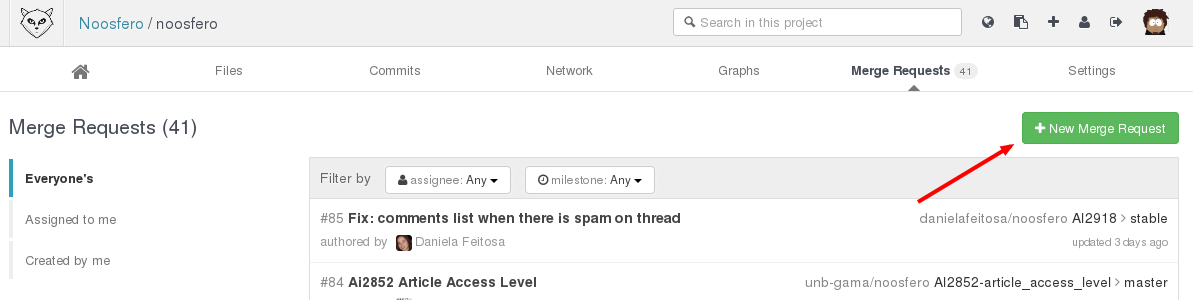
\includegraphics[scale=0.4]{gitlab-new-merge-request.png}
\caption{Novo merge request no Gitlab}
\label{fig:gitlab-new-merge-request}
\end{figure}

\subsubsection{Lista de verificação de revisão de código}

Esta lista de verificação é seguida durante a revisão do seu patch, por isso é
interessante você seguir essa verificação antes de submeter o seu patch. Essa
lista não é definitiva, e certamente vai crescer com o tempo.

\begin{itemize}
  \item aspectos gerais
  \begin{itemize}
    \item seguir o estilo de indentação já utilizado (2 espaços)
    \item o patch não deve conter espaços em branco à direita (git show ou git
      diff irá destacá-los se o recurso de cores estiver habilitado)
    \item o patch deve identificar um ActionItem em sua mensagem de log
    \item seja consistente. Se vocês fez algo de uma forma em um lugar, faça
      da mesma forma em todos os lugares
  \end{itemize}
  \item migrations
  \begin{itemize}
    \item quando uma nova coluna é adicionada e ela tem um valor padrão,
      garanta que os registros existentes serão atualizados para ter este
      valor padrão (exemplo: execute("update TABLE set NEWCOLUM =
      DEFAULTVALUE")). Isso parece redundante, mas nem todos os sistemas de
      banco de dados aplicam o valor padrão de uma nova coluna para os
      registros existentes
  \end{itemize}
  \item models: toda a lógica da aplicação deve estar nos models. Validações
    de dados, restrições, operações de consulta ao banco de dados ou qualquer
    outra modificação devem estar nos models
  \item controllers: garanta que os controllers só façam o trabalho necessário
    para implementar a interação com usuário. Deixe todas as validações e
    outros tipos de lógica para serem implementadas nos models
  \item tests: evite escrever testes que levam muito tempo para executar;
    evite acessar o banco de dados (ou seja, salvar objetos nele), a menos que
    seja absolutamente necessário
\end{itemize}

\section{Convenções de codificação}

% http://noosfero.org/Development/CodingConventionsPt

\subsection{Geral}

\subsubsection{Indentação}

A identação é 2 espaços, para todas as linguagens.

\subsubsection{Evite usar return nos métodos}

Use

\begin{Verbatim}[frame=single,fontfamily=courier]
def method
  value
end
\end{Verbatim}

ao invés de

\begin{Verbatim}[frame=single,fontfamily=courier]
def method
 return value
end
\end{Verbatim}

\subsubsection{Acesse métodos de instancia usando self.}

O uso de {\it self.method\_name} ao invés de {\it method\_name} deixa claro que
é algo de instancia, não uma variável.

Também, para métodos {\it setters}, se omitimos o {\it self.} poderá levar a
um erro pois irá criar uma variável ao invés de chamar o método de instancia.

Quando um método tem argumentos, sempre use parenteses na sua declaração

\subsection{Models}

\begin{itemize}
  \item relacionamentos (has\_many, belongs\_to, etc) e comportamentos
    (acts\_as\_*)
  \item atributos virtuais, se necessário
  \item validações
  \item lógica de negócio em geral
\end{itemize}

\subsection{Controllers magros, models gordos}

\begin{itemize}
  \item sempre que você escrever um método com mais que 5 linhas em um
    controller, considere mover esta lógica pra um model
  \item NUNCA referencie nada além de @variables dentro de templates (.rhtml)
\end{itemize}

\subsection{Testando}

\begin{itemize}
  \item teste toda validação que você tenha adicionado ao model
  \item adicione um teste ao seu conjunto de testes unitários que valide todos
    os dados nas fixtures através do ActiveRecord, a menos que você esteja
    utilizando fixtures) individuais como dados inválidos para testes. Nomeie
    seus dados inválidos nas \_fixtures com o prefixo "invalid\_"
  \item todo model deve ter testes unitários
  \item todo controller deve ter testes funcionais. Ao menos um teste para
    cada action
  \item cada estória de usuário deve ter um ou mais testes de integração
  \item relatórios do Rcov devem apresentar 100\% de cobertura de tudo
\end{itemize}

\section{Plugins Noosfero}

Guia de desenvolvimento de Plugins Noosfero.

% http://noosfero.org/Development/PluginsArchitecturePt

\subsection{Ativação de plugins}

A ativação de plugins funciona em duas etapas. Como os plugins serão mantidos
dentro da árvore do Noosfero, todos eles estarão disponíveis dentro da pasta
"plugins". O primeiro passo é executar o script {\it noosfero-plugins}. Com este
script você será capaz de gerenciar os plugins da sua instalação Noosfero.
Para ver as opções do script execute:

\begin{Verbatim}[frame=single,fontfamily=courier]
$ script/noosfero-plugins
(informações interessantes serão mostradas)
\end{Verbatim}

Para ativar um plugin, rode:

\begin{Verbatim}[frame=single,fontfamily=courier]
$ script/noosfero-plugins enable PLUGIN
\end{Verbatim}

Para ativar todos os plugins, rode:

\begin{Verbatim}[frame=single,fontfamily=courier]
$ script/noosfero-plugins enableall
\end{Verbatim}

Isso vai tornar o código do plugin disponível para ser carregado quando o
Noosfero for iniciado.

Os plugins são ativados também por {\it environment} (ambiente) já que o
Noosfero suporta múltiplos ambientes por instancia. A segunda etapa é ativar o
plugin usando uma conta de administrador. Acesse "/admin/plugins" e marque o
plugin como ativo.

\subsection{Estrutura Básica}

A estrutura de plugins do Noosfero é construída sobre um paradigma baseado em
eventos. O que isso significa? Isso significa que Noosfero dispara um evento
em um determinado ponto e todos os plugins interessados naquele
evento é capaz de agir. Então, cada novo evento deve ser bem documentado, para
que cada novo plugin possa definir suas ações adequadamente. Esses eventos são
chamados de {\it hotspots}.

Quando se trata de plugins, Temos 2 papéis básicos

\begin{itemize}
  \item Desenvolvedor Noosfero
  \item Desenvolvedor de Plugins
\end{itemize}

Cada um tem preocupações muito diferentes, mas no final o trabalho de ambos
serão combinados, para que haja consistência entre o que está sendo
desenvolvido.

\subsection{Visão do desenvolvedor Noosfero}

Antes de tudo, vamos dar uma olhada no lado do desenvolvedor Noosfero durante
a criação de um plugin. Antes da criação de qualquer plugin, este
desenvolvedor deve criar os hotspots para que os plugins possam se registrar e
começar a adicionar recursos interessantes ao Noosfero.

\subsubsection{Definindo hotspots}

Como dito antes, os eventos que são disparados aos plugins são chamados de
hotspots. Estes são os pontos onde os plugins podem fazer alguma ação. Para
definir um hotspot o desenvolvedor deve definir 4 pontos importantes:

\begin{itemize}
  \item Interface do Plugin
  \item A interpretação do lado do Noosfero
  \item Variáveis de contexto
  \item Testar os hotspots (os testes devem sempre estar lá!)
\end{itemize}

{\bf Interface do Plugin}

Para criar um novo evento, antes de tudo, deve-se criar um método na classe
Noosfero::Plugin que irá funcionar como interface entre o Noosfero e os
plugins. Este método deve ter uma breve documentação com a sua descrição e o
formato do valor de retorno. Este método deve retornar nil. Os plugins que
queiram se registrar para este evento deve sobrescrever este método de acordo
com as suas especificações. Vamos mostrar um exemplo implementado no plugin
Mezuro (o primeiro plugin do Noosfero):

lib/noosfero/plugin.rb
\begin{Verbatim}[frame=single,fontfamily=courier]
# -> Adds buttons to the control panel
# returns = { :title => title, :icon => icon, :url => url }
# title = name that will be displayed.
# icon = css class name (for customized icons include them in a css file).
# url   = url or route to which the button will redirect.
def control_panel_buttons
  nil
end
\end{Verbatim}

Como você pode ver, o desenvolvedor criou um novo evento chamado
"control\_panel\_buttons". Este evento permite que os plugins adicionem novos
botões ao painel de controle. Além disso, como uma boa prática, o
desenvolvedor especificou o formato do valor de retorno do evento. Cada novo
evento deve ser documentado com seus parâmetros e seus valores de retorno.
Neste caso, o formato do valor de retorno é um hash contendo um título, um
ícone e uma URL para onde o botão irá redirecionar. Lembre-se sempre de
definir valores de retorno de uma forma declarativa.

Note que o nome do evento é na forma plural. Isso é o padrão para os nomes dos
eventos. Os plugins podem retornar uma única resposta ou uma lista deles. Mas
não se preocupe, todas essas coisas são tratadas no manager. Apenas lembre-se
sempre de pluralizar os seus eventos.

{\bf Interpretação do lado do Noosfero}

Este é o ponto onde o desenvolvedor deve tratar a informação do plugin. Após a
definição do evento, o desenvolvedor deve tratar todos os plugins registrados
para o evento no local correto.

Para lidar com isso, o Noosfero implementa um Manager. Este manager é
recarregado a cada novo {\it request} com novas instâncias de cada plugin. Você pode
acessar este manager em cada view ou controller através da uma variável
@plugins. Para tornar mais fácil a vida do desenvolvedor, foi criado um método
para este manager chamado map. Esse método recebe um símbolo especificando o
evento que deve ser alertado e retorna uma lista com as respostas de todos os
plugins registrados para ele. Vamos ver como isso é feito com o evento
"control\_panel\_buttons" que vimos no último exemplo.

app/views/profile\_editor/index.rhtml
\begin{Verbatim}[frame=single,fontfamily=courier]
<% @plugins.map(:control_panel_buttons).each do |button| %>
<%= control_panel_button(button[:title], button[:icon], button[:url]) %>
<% end %>
\end{Verbatim}

Então, aqui o desenvolvedor dispara o evento com o método map e este método 
retorna todas as respostas dos plugins registrados para esse evento. Com esta 
lista, o desenvolvedor cria todos os botões que cada plugins especifica.

{\bf Variáveis de contexto}

A infraestrutura de plugins do Noosfero oferece uma variável com algumas
informações importantes sobre o contexto em que o evento foi disparado. Esta
informação é acessível aos plugins para que eles possam analisar o contexto
antes de definir o que fazer. As informações básicas existentes hoje são:
profile, request, response, environment e params. Se for necessário, você pode
definir novas informações no arquivo "lib/noosfero/plugin/context.rb".
Lembre-se que todo esta informação pode ser acessada a partir do controller.

{\bf Testando os hotspots}

O desenvolvido do Noosfero é guiado por testes (TDD), por isso precisamos
testar cada pequena parte. Isto não é diferente para a infraestrutura de
plugins. Além dos testes funcionais e de unidade que você pode precisar criar
ao definir um novo evento, o Noosfero oferece uma maneira fácil de lidar com
os testes de integração cucumber para os eventos do lado do Noosfero. No
exemplo que vimos antes, o desenvolvedor criou a interface para os plugins
adicionar novos botões ao painel de controle. Vamos ver como podemos fazer um
teste simples para verificar se este novo recurso está funcionando como
esperado.

\begin{Verbatim}[frame=single,fontfamily=courier]
Background:
  Given the following plugin
    | klass       |
    | TestPlugin  |
  And the following events of TestPlugin
    | event                 | body                                                                  |
    | control_panel_buttons | lambda { {:title => 'Test plugin button',
    :icon => '', :url => ''} }  |
 
Scenario: a user must see the plugin's button in the control panel if\
          the plugin is enabled
  Given plugin TestPlugin is enabled on environment
  And I go to Joao Silva's control panel
  Then I should see "Test plugin button"
 
Scenario: a user must not see the plugin's button in the control panel\
          if the plugin is disabled
  Given plugin TestPlugin is disabled on environment
  And I go to Joao Silva's control panel
  Then I should not see "Test plugin button"
\end{Verbatim}

Vamos ver isso por partes.

Antes de tudo, você vê que o Noofero oferece o passo "the following plugin",
onde é possível definir quais plugins estarão habilitados no ambiente de
testes. Você só precisa definir o nome da classe do plugin.

Após criar o plugin, você pode especificar cada evento para o qual o plugin
está registrado como informado no passo "following events of TestPlugin". Você
deve definir o nome e o corpo do evento. Note que o corpo deve ser um bloco
de código.

O último recurso é o passo "plugin <plugin-class-name> is enabled/disabled on
environment".

É isso aí. Agora você tem um plugin básico para fazer qualquer teste que você
precisa em seus novos eventos.

\subsection{Visão do desenvolvedor de Plugins}

Agora vamos dar uma olhada no lado do desenvolvedor de plugins. Nesta parte,
vamos estudar de perto os seguintes pontos da criação de um plugin.

\subsubsection{Como criar um Plugin Noosfero}

Há uma estrutura importante dentro do diretório plugin. Você não deve se
preocupar com isso. Apenas execute:

\begin{Verbatim}[frame=single,fontfamily=courier]
$ script/noosfero-plugins new cool_feature
\end{Verbatim}

O CoolFeaturePlugin será criado e ativado. Você deve reiniciar o servidor
Noosfero. Você irá encontrar o código gerado em
plugin/cool\_feature/lib/cool\_feature\_plugin.rb com este conteúdo.

\begin{Verbatim}[frame=single,fontfamily=courier]
class CoolFeaturePlugin < Noosfero::Plugin
 
  def self.plugin_name
    # FIXME
    "Cool Feature" # you can change it freely,
                   # but the word "plugin" is overabundant
  end
 
  def self.plugin_description
    # FIXME
    _("A plugin that does this and that.")
  end
 
end
\end{Verbatim}

Para facilitar o entendimento dos próximos passos, iremos usar como exemplo o
primeiro plugin Noosfero, o plugin Mezuro.

\subsubsection{Definição}

Agora você pode estar dizendo: "Então aqui estamos nós, os desenvolvedores do
Noosfero criaram muitos hotspots legais e agora eu quero criar um novo plugin
que irá utilizar vários deles, o que devo fazer?".

Vamos lá:

\begin{itemize}
  \item Crie uma pasta com o nome do seu plugin.
  \item Dentro desta pasta cria um aquivo chamado "init.rb" e uma pasta
    chamada "lib".
  \item Dentro da pasta "lib" crie um arquivo chamado
    "<your-plugin-name>\_plugin.rb". Em nosso caso, este arquivo será chamado
    "mezuro\_plugin.rb".
  \item Agora abra o arquivo "init.rb".
  \item Dentro desse arquivo escreva "require '<your-plugin-name>\_plugin'".
    No nosso caso, "require 'mezuro\_plugin'". Este arquivo de inicialização
    será chamado na inicialização do Noosfero. Portanto, é uma boa idéia para
    separar o carregamento do seu plugin de definição dele.
  \item Agora que carregamos o plugin, vamos especificar ele. Abra o arquivo
    'lib/<your-plugin-name>\_plugin.rb'.
\end{itemize}

A infraestrutura de plugins do Noosfero oferece a possibilidade de especificar
algumas meta-informações. Hoje, as meta-informações suportados são name e
description. Estas informações serão utilizadas para descrever o seu plugin no
Noosfero, é muito importante defini-los. Para checar todas as meta-informações
disponíveis no Noosfero dê uma olhada no arquivo 'lib/noosfero/plugin.rb'. No
caso do Mezuro, definimos as seguintes meta-informações.

\begin{Verbatim}[frame=single,fontfamily=courier]
def self.plugin_name
  "Mezuro"
end
 
def self.plugin_description
  _("A metric analizer plugin.")
end
\end{Verbatim}

NOTA: o '\_()' é usado para traduzir o texto para os idiomas disponíveis.

\subsubsection{Plugins e extensão do core}

{\bf Eventos}

Após definir as meta-informações, é hora de lidar com os hotspots. Para
registar o plugin a um evento, basta definir um método sobrescrevendo o evento
para o qual você deseja. Neste caso, vamos usar o evento
"control\_panel\_buttons". Antes de qualquer coisa, devemos ver a definição do
formato do evento. Vamos dar uma olhada no arquivo "lib/noosfero/plugin.rb".

lib/noosfero/plugin.rb
\begin{Verbatim}[frame=single,fontfamily=courier]
# -> Adds buttons to the control panel
# returns = { :title => title, :icon => icon, :url => url }
# title = name that will be displayed.
# icon = css class name (for customized icons include them in a css file).
# url = url or route to which the button will redirect.
def control_panel_buttons
  nil
end
\end{Verbatim}

Como esperávamos, o desenvolvedor criou um hotspot bem documentada. Agora
sabemos que o nosso plugin deve retornar um hash contendo o título do botão, o
nome da classe css para definir o ícone do nosso botão e uma url para onde o
botão irá redirecionar. Muito claro! Este é o poder da definição declarativa.
Nós só devemos nos preocupar com as informações do botão e não em como ele vai
ser implementado. Então, vamos ver como Mezuro implementa este hotspot.

\begin{Verbatim}[frame=single,fontfamily=courier]
def control_panel_buttons
  if context.profile.community?
   { :title => 'Mezuro projects', :icon => 'mezuro', 
    :url => {:controller => 'mezuro_plugin_myprofile', :action => 'index'}}
  end
end
\end{Verbatim}

Aqui temos algumas novidades.

A primeira é o contexto variável. Esta variável é oferecida pelo Noosfero para
os plugins contendo algumas informações sobre o contexto de onde o evento está
sendo acionado. Neste exemplo vamos verificar se o perfil é uma comunidade
antes de adicionar o novo botão. Hoje, as informações disponíveis são:
profile, request, response, environment e params. Para verificar as
informações disponíveis dê uma olhada em "lib/noosfero/plugin/context.rb". Se
precisar de alguma informação que não está disponível no contexto, contate
qualquer desenvolvedor Noosfero ou envie um patch.

A segunda é a rota que é usada na variáve :url. Esta rota é uma rota de
plugin. Vamos discutir melhor este ponto na seção "Controladores e rotas".

Observe que, em todos esses eventos, o plugin pode retornar uma única resposta
ou uma lista deles. É por isso que cada evento deve estar no plural. Isso tudo
é tratado no Manager.

Agora estamos prontos! Com apenas esses passos você tem um plugin que adiciona
um novo botão ao painel de controle das comunidades! Mas o que este botão faz?
Para onde ele redireciona? O que podemos fazer com ele? Tenha calma. Iremos
abordar todas estas questões nas etapas seguintes.

{\bf Extendendo classes do core}

Em muitos momentos, o seu plugin vai querer estender ou redefinir
características dos models do core. Normalmente, você deve fazer isso através
de um hotspot definido, mas às vezes um hotspot é muito exagero para as coisas
mais simples ou as vezes não é suficiente para coisas maiores. Nestes casos,
você pode estender os models do core, adicionando essas novas definições na
pasta "ext", que deve ser criada dentro da pasta "lib". Por exemplo, se
quiséssemos extender o model Article, só precisamos criar o arquivo
lib/ext/article.rb com um conteúdo mais ou menos assim.

\begin{Verbatim}[frame=single,fontfamily=courier]
require_dependency 'article'
 
class Article
  def hit_with_mezuro_plugin_extension
    hit_without_mezuro_plugin_extension
    puts "This is the hit new extension!"
  end
  alias_method_chain :hit :mezuro_plugin_extension
 
  def mezuro_plugin_new_method
    puts "Also adding a new method!"
  end
end
\end{Verbatim}

Em primeiro lugar, observe que precisamos citar o model article na primeira
linha. Isso é necessário, pois o Rails usa lazy loading para o carregamento
de classes do core, por isso você deve explicitamente carregar o model article para
garantir que a extensão funciona corretamente. O 'require\_dependency' é útil
para evitar múltiplas carregamentos do model.

Depois disso, nós reescrevemos a forma de execução encadeando um código que
irá incluir um novo método no model article. Note que tanto a extensão
encadeada quanto o nome do método são prefixados com o nome do plugin. Isso é
importante para evitar conflitos de nome. Você pode estender os models com
tudo que um model permite fazer, mas lembre sempre: "grandes poderes trazem
grandes responsabilidades". Utilize este recurso com cuidado e lembre-se de
usar o princípio da namespacing sempre que você julgar necessário.

{\bf Escopo}

Como o código dos plugins (seja Ruby, JS ou CSS) é carregado em cada request,
é importante o escopo para que estes códigos não entrem em conflito com os
outros. Para mais explicações, considere o nome do plugin MyPlugin
(my\_plugin).

{\it Ruby}

Prefixe nomes de classes/módulos com MyPlugin ou coloque no namespace da classe.

{\it Javascript}

Use protótipo JS para definir objetos:
\begin{Verbatim}[frame=single,fontfamily=courier]
myplugin = {

  value: 1,

  f: function() {
    console.log('hello');
  },

}
myplugin.f();
\end{Verbatim}

{\it CSS}

Prefixe nomes de classe ou use seletor de pai para evitar conflitos com outros
estilos.

\begin{Verbatim}[frame=single,fontfamily=courier]
#myplugin-parent .button {
}
.myplugin-button {
}
\end{Verbatim}

{\bf Adicionando coisas ao user data}

Plugins também podem adicionar valores extras para o hash utilizado no user
data, que é carregado via Ajax em cada carregamento da página.

\subsubsection{Tabelas e registros}

{\bf Migrations}

Se o seu plugin precisa criar novas tabelas, o Noosfero oferece suporte a
isso. Para adicionar novas migrations defina elas (como em uma aplicação Rails
qualquer) dentro de uma pasta "db/migrate/". Você deve observar três pontos
importantes:

\begin{itemize}
  \item Todas as suas migrations não devem depender das migrations do core do
    Noosfero.
  \item Todas as suas migrations devem usar o formato com data e hora antes do
    nome da do arquivo para evitar conflitos com outras migrations. Ex:
    20101209151530\_create\_projects.rb
  \item Toda nova tabela que você criar deve usar "<plugin-name>\_plugin".
    Isso vai evitar conflitos com outras tabelas. No caso do Mezuro,
    precisamos criar duas novas tabelas: projexts e metrics. (migrations
    abaixo)
\end{itemize}

\begin{Verbatim}[frame=single,fontfamily=courier]
class CreateProjects < ActiveRecord::Migration
  def self.up
    create_table :mezuro_plugin_projects do |t|
      t.string      :name
      t.string      :identifier
      t.string      :personal_webpage
      t.text        :description
      t.string      :repository_url
      t.string      :svn_error
      t.boolean     :with_tab
      t.references  :profile
 
      t.timestamps
    end
  end
 
  def self.down
    drop_table :mezuro_plugin_projects
  end
end

class CreateMetrics < ActiveRecord::Migration
  def self.up
    create_table :mezuro_plugin_metrics do |t|
      t.string  :name
      t.float   :value
      t.integer :metricable_id
      t.string  :metricable_type
 
      t.timestamps
    end
  end
 
  def self.down
    drop_table :mezuro_plugin_metrics
  end
end
\end{Verbatim}

Descarte as mudanças no db/schema.rb usando git checkout, pois as migrations
dos plugins são executadas dependendo do plugin está ou não ativo.

Atenção: evite a todo custo adicionar novos atributos a tabelas existentes.
Suponha que você deseja adicionar o atributo foo\_id a tabela de profiles para
ser capaz de adicionar uma associação belongs\_to ao Profile. Em vez disso,
adicione a profile\_id a tabela foos e adicione uma relação has\_one ao Profile.

{\bf Models}

Definir models para o seu plugin é muito importante quando você tem um plugin
que lida com aspectos complexos. Então, vamos ver como você pode definir novos
modelos que irão trabalhar em conjunto com Noosfero.

Antes de tudo, todos os seus models devem estar dentro de um módulo
chamado "<your-plugin-name-camelcased>Plugin". No caso do Mezuro seria
"MezuroPlugin". Isto é necessário porque temos de garantir que seus novos
models não entrem em conflito com outros plugins, ou mesmo com os models do
core do Noosfero. Então, se você precisa de novos models, crie uma nova pasta
chamada "<your-plugin>\_plugin" (mezuro\_plugin) dentro da pasta "lib". Dentro
desta nova pasta você deve definir todos os seus novos models. O plugin Mezuro
precisou criar um novo model chamado Project. Então criamos o arquivo
"lib/mezuro\_plugin/project.rb". Para especificar que este model está dentro do
módulo MezuroPlugin devemos defini-lo desta maneira:

\begin{Verbatim}[frame=single,fontfamily=courier]
class MezuroPlugin::Project < ActiveRecord::Base
end
\end{Verbatim}

Mas isso não é suficiente. Como você precisa de um novo model, você
provavelmente vai precisar criar uma nova tabela para este model e como
descrito na seção "Migrations" todas as tabelas dos plugins ficam no namespace
"<plugin-name>\_plugin". O problema é que o ActiveRecord::Base do Rails tem a
sua própria maneira de mapear o nome\_classe para nome de tabela. Então o
Noosfero criou uma nova ActiveRecord::Base que é exatamente igual mas redefine
o método table\_name. Assim, todos os seus models em vez de herdar de
ActiveRecord::Base devem herdar de Noosfero::Plugin::ActiveRecord. Em seguida
o novo model Project que estamos criando seria assim.

\begin{Verbatim}[frame=single,fontfamily=courier]
class MezuroPlugin::Project < Noosfero::Plugin::ActiveRecord
end
\end{Verbatim}

Lembre-se que sempre que for preciso acessar este model de outros lugares é
preciso se referir a ele como MezuroPlugin::Project em vez de apenas Project.

\subsubsection{Controllers e rotas}

A infra-estrutura de plugins oferece uma maneira genérica para fornecer rotas
para os plugins baseados na pasta em que o controller do plugin é colocado. Há
quatro pastas disponíveis, cada uma definindo uma rota base. Assim, para criar
um controller você deve criar a pasta "controllers" e dentro desta pasta criar
a pasta apropriada que define o contexto de seu controller e dentro desta
parta criar o arquivo do controller. O nome do arquivo do controller deve
estar no seguinte formato:
<plugin-name>\_plugin\_<desired-controller>\_controller.rb. Estas rotas são como
se segue (usando o Mezuro como exemplo).

Rota de Profile
\begin{itemize}
  \item Contexto: profile
  \item Acesso: public
  \item Pasta: mezuro/controllers/profile
  \item Rota: /profile/:profile/plugins/mezuro/<controller-name>/:action/:id
  \item Herança do Controller: ProfileController
\end{itemize}

Rota de Myprofile
\begin{itemize}
  \item Contexto: profile control panel
  \item Acesso: profile edition permission
  \item Pasta: mezuro/controllers/myprofile
  \item Rota: /myprofile/:profile/plugin/mezuro/<controller-name>/:action/:id
  \item Herança di Controller: MyprofileController
\end{itemize}

Rota de Admin
\begin{itemize}
  \item Contexto: administration
  \item Acesso: environment edition permission
  \item Pasta: mezuro/controllers/admin
  \item Rota: /admin/plugin/mezuro/<controller-name>/:action/:id
  \item Herança do Controller: AdminController
\end{itemize}

Rota Pública
\begin{itemize}
  \item Contexto: environment
  \item Acesso: public
  \item Pasta: mezuro/controllers/public
  \item Rota: /plugin/mezuro/<controller-name>/:action/:id
  \item Herança do Controller: PublicController
\end{itemize}

Antes destas rotas genéricos, haviam apenas 3 controllers disponíveis para os
plugins usar (como descrito abaixo). Estas rotas ainda estão disponíveis,
embora obsoleta agora. O Noosfero oferece 3 rotas para os plugins: profile,
myprofile e environment. Estas rotas são como se segue (usando Mezuro como
exemplo).

Rota de Profile
\begin{itemize}
  \item Contexto: profile
  \item Acesso: public
  \item Rota: /profile/:profile/plugins/mezuro/:action/:id
    \{:controller=>"mezuro\_plugin\_profile"\}
\end{itemize}

Roda de Myprofile
\begin{itemize}
  \item Contexto: profile control panel
  \item Acesso: profile edition permission
  \item Rota: /myprofile/:profile/plugin/mezuro/:action/:id
    \{:controller=>"mezuro\_plugin\_myprofile"\}
\end{itemize}

Rota de Environment
\begin{itemize}
  \item Contexto: environment
  \item Acesso: environment edition permission
  \item Rota: /plugin/mezuro/:action/:id =>
    \{:controller=>"mezuro\_plugin\_environment"\}
\end{itemize}

Com estas rotas, você pode usar qualquer um desses três controllers de acordo
com a situação. Para usá-los, crie a pasta "controllers" e dentro desta pasta
crie o arquivo do controller. O nome do arquivo do controller deve estar no
seguinte formato: <plugin-name>\_plugin\_<desired-controller>\_controller.rb. No
caso do Mezuro, foi preciso usar o controller myprofile, por isso criamos o
arquivo "controllers/mezuro\_plugin\_myprofile\_controller.rb". Vamos dar uma
olhada neste controller.

\begin{Verbatim}[frame=single,fontfamily=courier]
class MezuroPluginMyprofileController < MyProfileController
  append_view_path File.join(File.dirname(__FILE__) + '/../views')
 
  def index
    @projects = MezuroPlugin::Project.by_profile(profile)
  end
 
end
\end{Verbatim}

Olhando a primeira linha, você pode ver que o controller deve herdar de
respectivo NooferoController da seguinte forma:

\begin{itemize}
  \item myprofile => MyProfileController 
  \item profile => ProfileController 
  \item admin => AdminController 
  \item public => PublicController 
\end{itemize}

A segunda linha é a única forma de relacionar controllers e views até o
momento. Nós planejamos corrigir isto mas, até o momento, você deve adicionar
esta linha em todos os seus controllers.

O resto é quase o mesmo que um controller comum. Note que, como dito na seção
sobre "Models", é preciso acessar os models através do namespace de módulo
(MezuroPlugin::Project).

Lembra do botão criado no evento "control\_panel\_buttons"? Vamos dar uma
olhada nele novamente.

\begin{Verbatim}[frame=single,fontfamily=courier]
def control_panel_buttons
  if context.profile.community?
   { :title => 'Mezuro projects', :icon => 'mezuro',
   :url => {:controller => 'mezuro_plugin_myprofile', :action => 'index'}}
  end
end
\end{Verbatim}

Agora o novo botão irá redirecionar para o "index" do controller! O que você
acha de adicionar alguma visualização para este action agora? Verifique a
seção "Views".

\subsubsection{Views}

As views de seu plugin vão funcionar exatamente da mesma forma que outras
views. Você só precisa criar uma pasta chamada "views" e dentro dela criar uma
nova pasta para cada controller que você tiver. Fácil, não?

Portanto, se queremos adicionar uma view para a action "index" do nosso
controller "MezuroPluginMyProfileController" nós só precisamos criar a pasta
"views/mezuro\_plugin\_myprofile" e dentro dela criar o arquivo
"index.html.erb". A view vai funcionar como você já sabe. Aqui está um exemplo
simples.

\begin{Verbatim}[frame=single,fontfamily=courier]
<h1> <%= _("%s's Mezuro projects") % profile.name %>  </h1>
 
<% if @projects.blank? %>
  <%= _("%s has no projects registered.") % profile.name %>
<% else %>
  <%= _('Projects: ') %>
  <ul>
    <% @projects.each do |project|   %>
      <li><%= project.name %></li>
    <% end %>
  </ul>
<% end %>
\end{Verbatim}

Note que essa view será executada no escopo do MyProfileController, assim
temos acesso a coisas do profile. Outra coisa a ter em mente é que a página
estará no contexto deste controller também, então sua view será renderizada
por algum template adequado.

Pronto! Agora, quando o usuário abrir o painel de controle de uma comunidade
ele vai ver o seu botão e quando clicar nele, será redirecionado para uma
página que mostra todos os projetos desse profile. Muito legal!

{\bf Traduções}

As traduções são adicionaras junto ao código de tradução do core no diretório
po.

1) Defina o os valores que serão retornados no hash definindo o método
user\_data\_extras no seu plugin exemplo.

\begin{Verbatim}[frame=single,fontfamily=courier]
def user_data_extras
  { :test => 'This is a test' }
end
\end{Verbatim}

Então, a chave "test" estará disponível no hash com o valor "This is a test".
Você pode adicionar quantos pares chave/valor quiser.

2) Lidar com os dados.

Para lidar com os dados retornados, você precisa tratar o evento userDataLoaded no seu plugin, exemplo:

\begin{Verbatim}[frame=single,fontfamily=courier]
<script type="text/javascript">
  jQuery(window).bind("userDataLoaded",
     function(event, data) { alert(data.test); });
</script>
\end{Verbatim}

Quando o usuário visita uma página que contém este script, um alerta será
exibido com a mensagem "This is a test".

\subsubsection{Arquivos públicos}

Você pode adicionar um diretório public ao seu plugin, onde você pode
adicionar folhas de estilo, imagens e outros arquivos a serem acessados
diretamente pelos clientes.

Para habilitar isso você precisa criar um link simbólico para a pasta public
do seu plugin dentro de noosfero\_root/public/plugins, mas não se preocupe, o
"noosfero-plugins enable" fará todo o trabalho necessário para você.

\begin{Verbatim}[frame=single,fontfamily=courier]
script/noosfero-plugins enable some_plugin
\end{Verbatim}

Então você pode acessar os arquivos do seu plugin como:

\begin{Verbatim}[frame=single,fontfamily=courier]
http://localhost:3000/plugins/some_plugin/some-file
\end{Verbatim}

Isto é necessário para o método {\it stylesheet?}. Quando retorna true, o
arquivo some\_plugin/public/style.css será adicionado ao cabeçalho header.

\subsubsection{Testes}

A estrutura de testes segue a mesma estrutura dos testes do lado do Noosfero.
Então apenas coloque os testes nos diretórios test/\{units,funcionals\} e
features. Como de costume, os testes carregam helpers (exemplo: test\_helper.rb
para testes unitários). Para o seu plugin você pode definir seu próprio
test\_helper e ele pode carregar o test\_helper do core Noosfero.

{\bf Tasks}

O Noosfero oferece algumas tasks rake para você executar os testes do plugin sem
precisar rodar todos os testes do Noosfero. Como as tasks são geradas
dinamicamente, pode haver alguma dificuldade ao entender o código que faz
isto. (Mas se você quiser dê uma olhada em: lib/tasks/plugins\_tasks.rb). As
tasks são as seguintes.

(Note: todos os comandos abaixo tem um 'rake' antes)
\begin{itemize}
  \item test:noosfero\_plugins AND test:noosfero\_plugins:available - 
    Executa todos os testes de plugins
  \item test:noosfero\_plugins:enabled -
    Executa todos os testes de plugins ativados
  \item test:noosfero\_plugins -
    Executa todos os testes de um plugin específico
\end{itemize}

Todas essas tasks podem ter units/functionals/integration ao final para
especificar o tipo dos testes. Então, para rodar todos os testes unitários
para todos os plugins ativados você pode rodar por exemplo:

rake test:noosfero\_plugins:enabled:units

\subsubsection{Dependencias and Instalação}

O Noosfero também tem uma forma esperta para permitir plugins definir seu
próprio processo de instalação e dependências. Para tal, existe,
respectivamente, os arquivos install.rb e dependencies.rb. O install.rb é
código ruby onde o plugin recebe tudo necessário para preparar seu ambiente, e
assim estar pronto para execução, ao menos no ambiente de teste e
desenvolvimento. O dependencies.rb tenta carregar cada dependência do plugin
afim de permitir o Noosfero saber se o plugin está pronto para executar após
sua instalação.

O arquivo install.rb é executado sempre que o plugin é ativado, então é
importante que seu processo seja Idempotente. Aqui vão alguns exemplos do
install.rb e dependencies.rb.

install.rb
\begin{Verbatim}[frame=single,fontfamily=courier]
system "gem install --user-install net-ldap -v 0.3.1"
puts "\nWARNING: This plugin is not setting up a ldap test\
     server automatically.
Some tests may not be running. If you want to fully test this\
     plugin, please
setup the ldap test server and make the proper configurations on
fixtures/ldap.yml.\n\n"
\end{Verbatim}

dependencies.rb
\begin{Verbatim}[frame=single,fontfamily=courier]
require 'rubygems'
require 'net/ldap'
\end{Verbatim}

\section{Comunidade Participa.br}

A comunidade envolvida ao projeto Perticipa.br está organizada através
das seguintes ferramentas:

\subsection{Lista de discussão participa-dev}

https://groups.google.com/forum/\#!forum/participa-dev

Toda comunicação do grupo envolvido com o projeto é feito via lista de
discussão, a lista participa-dev é o canal oficial para os envolvidos com a
criação e desenvolvimento do mesmo.

\subsection{Gitlab Wiki}

https://gitlab.com/participa/noosfero/wikis/home

No Wiki do Gitlab está sendo mantido toda informação sobre o andamento
do projeto, quem está fazendo o quê, cronogramas, reuniões, revisão de código,
etc.

\subsection{Gitlab Issues}

https://gitlab.com/participa/noosfero/issues

Todos os bugs encontrados no contexto do projeto Participa.br é registrado
aqui antes de ir parar no tracker oficial do Noosfero, alguns requisitos de
infra-estrutura ou mesmo sugestões de melhorias e implementações estão sendo
registradas de forma centralizadas aí.

\section{Plugins/módulos do Participa.br}

O portal de Participação Social (Participa.br) utiliza hoje os seguintes
plugins.

\begin{itemize}
  \item BreadcrumbsPlugin: Um plugin que adiciona um block para exibir o
    caminho da página sendo visualizada
  \item CommentGroupPlugin: Um plugin que mostra grupos de comentários em
    artigos por parágrafo ou trecho de texto
  \item CommunityBlockPlugin: Um plugin que adiciona um bloco para mostrar a
    descrição de uma comunidade
  \item CommunityTrackPlugin: Um plugin que adiciona um novo tipo de conteúdo
    para comunidades
  \item ContainerBlockPlugin: Um plugin que adiciona um bloco de blocos
  \item DisplayContentPlugin: Um plugin que adiciona blocos onde você pode
    escolher qualquer um dos seus conteúdos para mostrar
  \item DisplayContextContent: Um plugin que mostra conteúdo baseado no
    contexto da página
  \item PeopleBlockPlugin: Um plugin que adiciona um bloco de pessoas
  \item PgSearchPlugin: Motor de busca que usa a Busca Full-Text do Postgres
  \item RequireAuthToCommentPlugin: Exige que os usuários se autentiquem antes
    de postar comentários
  \item SpaminatorPlugin: Um plugin que busca e destrói spams
  \item StatisticsPlugin: Um plugin que adiciona um bloco para mostrar
    estatísticas por contexto da navegação
  \item SubOrganizationsPlugin: Um plugin que adiciona a possibilidade de
    grupos terem sub-grupos
  \item VideoPlugin: Um plugin que adiciona um bloco para adicionar vídeos do
    youtube, vimeo e html5
  \item WorkAssignmentPlugin: Novo tpo de conteúdo para organizações
\end{itemize}

Todos estes plugins são distribuídos junto ao código-fonte do Nosfero e podem
ser consultados na pasta "plugins/" na raiz do projeto Noosfero.

%% http://noosfero.org/Development/TrainingNoosferoPt
%% http://noosfero.org/Development/Localization
%% http://noosfero.org/Development/Profiling
%% http://noosfero.org/Development/Schroot
%% http://noosfero.org/Development/CreatingThemes
%% http://noosfero.org/Development/MonkeyPatch
%% http://noosfero.org/Development/Debug
%
%O Participa.br ...

\section{Fomento à formação de comunidade de desenvolvimento}

Uma das principais formas de fomento à comunidade de desenvolvedores do
Noosfero é promover eventos técnicos tipo "mão na massa", onde se estimula as
pessoas terem um contato inicial com o desenvolvimento do projeto, propiciando
um passo-a-passo que irá despertar o interesse de novos desenvolvedores.

\section{Considerações finais}

Neste documento foi apresentada um guia de codificação "coding guidelines"
para o desenvolvimento do código do portal objetivando o reaproveitamento de
código e o fomento à formação de comunidades em torno dos módulos, bem como
tutoriais para implementação local das soluções.

Lembramos que para tornar o Portal de Consulta Pública realmente um canal de
consulta e participação popular na discussão e na definição da agenda
prioritária do país, é necessário que além de documentação faça-se um esforço
de movimentar as pessoar fora do ambiente virtual, para que haja um
engajamento no uso e contribuição deste projeto de forma consistente e perene.

\vspace{1cm}

Sem mais nada a acrescentar, coloco-me à disposição.

\vspace{1cm}

\begin{minipage}{\textwidth}
  Brasília/DF, \DiaEntrega \ de \MesEntrega\\[1cm]
  \textbf{\MyName}\\
  \small Consultor do PNUD
\end{minipage}

%\newpage
%\appendix
%\appendixpage
%\section{Foo bar}
\label{foobar}

%\lstinputlisting{observatorio.rb}


\end{document}
